\documentclass{../../../lessonplan}
\renewcommand{\cflroot}{../../..}

\begin{document}

\lessonplantitle
    {UKS2-S1}
    {Upper Key Stage 2 Session 1}
    {What do we already know? Recap the Blockly commands previously encountered}

\preamble
    {
    \item Use the core programming commands appropriately to a visual language
    \item Understand the \keyword{repeat while} command
    }
    {
    \item Interactive White Board (IWB)
    \item Levels 51-60 in Rapid Router
    \item Resource sheet UKS2-S1-1
    \item UKS2 Levels Guide
    \item UKS2 Program Solutions Table
    \item STOP sign on A4 card (teacher made)
    \item LKS2 and UKS2 Assets - Blockly cards
    \item UKS2 Code Wall Cards
    }
    {
    \item move forwards, turn left, turn right
    \item repeat
    \item repeat until at destination
    \item repeat while not at destination (introduce this in preparation for Python)
    \item if ... else if ... else
    }

\begin{lessonplan}

\textbf{Explain to the children that in this block of work, they are going to learn how to write code for computer programs the way programmers in industry do.}

They will be using a language called Python which is used by lots of computer programmers.

Before that, it is important that everyone remembers the programming skills they have learnt using Blockly, so the first session will be about sharing what everyone knows.

Run through the Blockly vocabulary they have already come across, using the Blockly cars in the LKS2 and UKS2 Assets.

\keyquestion{Can you explain what these blocks of code will do using the programming language you have already learnt?}

Show Level 51 on the IWB.
Explain that they can only use a certain number of blocks, so there is an extra challenge. \textit{[fig S1.1]}

\fig{fig S1.1}{figS1.1.jpg}{1}

\subsection*{Independent activity}

Ask the children to work on Levels 51 to 56, individually if possible, so that you can assess their confidence and understanding in using the movement and repetition commands.

\subsection*{Mini review}

Discuss how they have done so far and choose some children to explain how they tackled a particular level.

\keyquestion{Can you explain how the \keyquestion{repeat until at destination} command works in Level 55?}

Introduce \keyword{repeat while not at destination} as an equivalent to \keyword{repeat until at destination}.

\fig{fig S1.2}{figS1.2.jpg}{1}

Illustrate this idea by playing a `repeat until the sign says STOP' game where children repeat a clapping or movement rhythm until you hold up a STOP sign.
Write the instruction `repeat until the sign says STOP' on the flipchart/board.

Rename the game `repeat while there is NOT a STOP sign showing', writing this on the flipchart and play again.

The class should see that the instructions work identically.

Explain that in Level 57 they have a \keyword{repeat while} block, rather than a \keyword{repeat until} block.

Display these code wall cards together for comparison.

Give the children a few minutes to discuss in pairs how they would write the program, and choose a pair to explain their thinking.

Ask the class to try Levels 57 and 58.
Those who complete these quickly can go on to Level 60.

Give them resource sheet UKS2-S1-1 to record their algorithm for Level 57, and explain that you will be discussing this at the end of the lesson. \textit{[fig S1.2]}

\subsection*{Share and review}

Look at Level 57 together on the IWB. \textit{[fig S1.3]}

\fig{fig S1.3}{figS1.3.jpg}{1}

Choose a child to come and explain how they programmed a solution.
Ask if anyone found a different solution.

Compare their solution with the model solution in the Program Solutions Table.

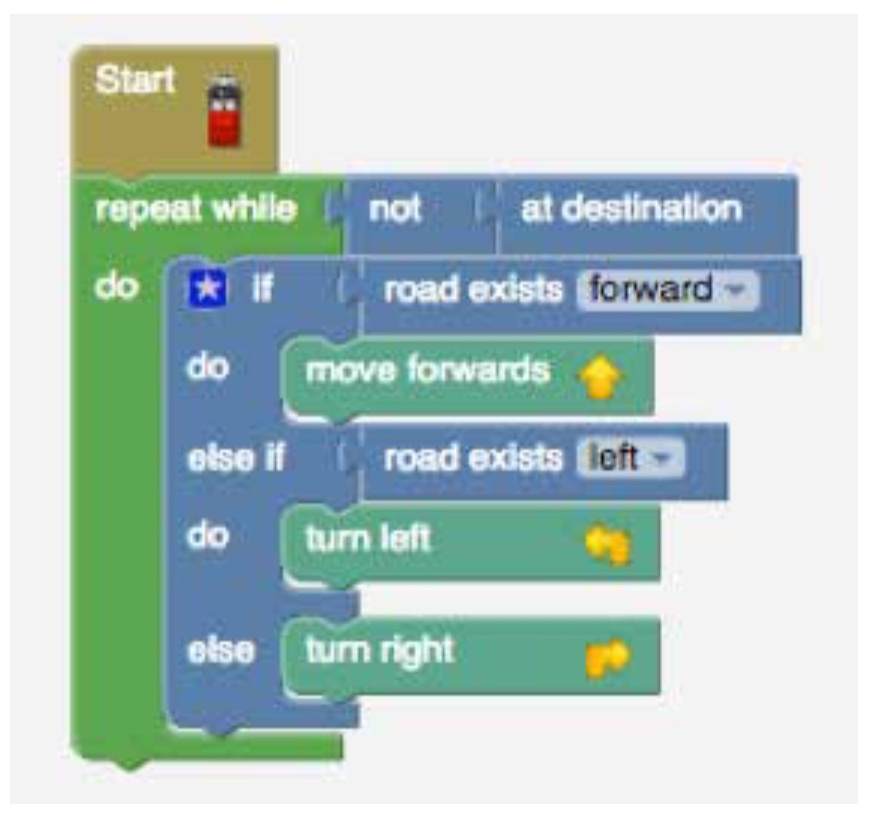
\includegraphics[width=\linewidth]{solution.jpg}

\keyquestion{Does it matter which order the \keyword{if} confidencestions are listed? Why not?}

\keyquestion{Is your solution as efficient? Can you explain how it works?}

Use this opportunity to assess children's understanding of the concept of selection.

Finish off by discussing what they have learnt in this session.


\end{lessonplan}

\end{document}
